\setchapterimage[3.5cm]{mma/crab-page}
\setchapterpreamble[u]{\margintoc}
\chapter{Summary and Future Outlook}
\labch{summary}
\begin{fquote}[Ambrose Bierce][The Cynic's Dictionary][1906] FUTURE, n. That period of time in which our affairs prosper, our friends are true and our happiness is assured.  
\end{fquote}

LSST

Ligo O4 + LIGO India + Kagra -> Many kilonovae -> Hubble constant, test general relativity, 

IceCube Gen2 + PeV band + KM3net + Baikal + P-One

Radio


\begin{marginfigure}
	\centering 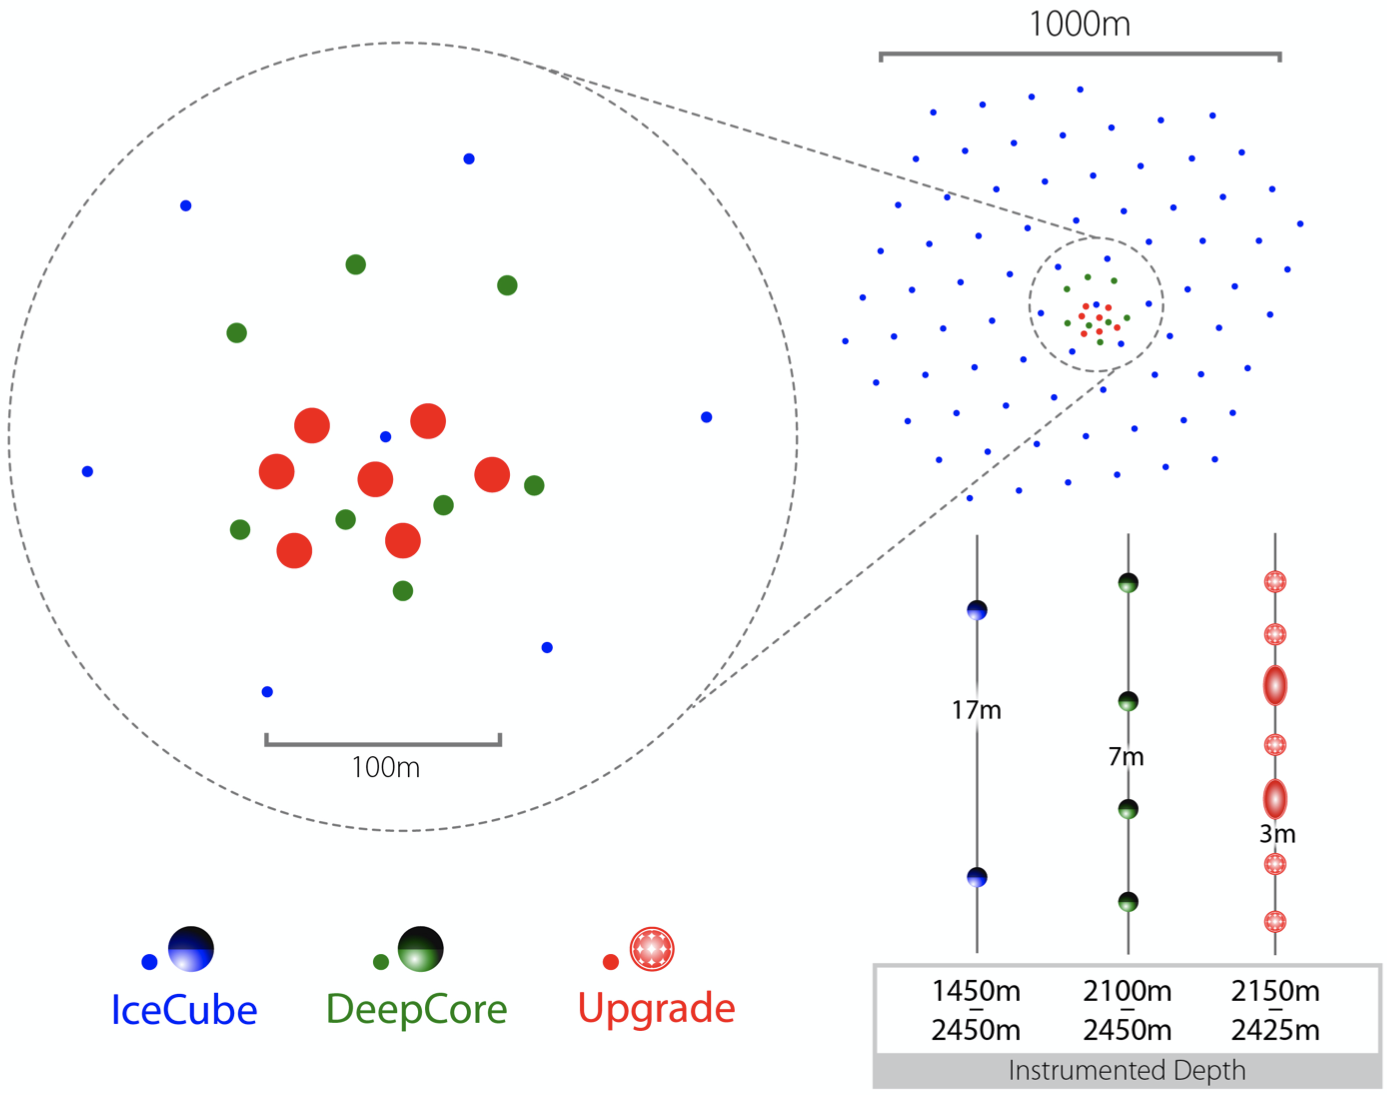
\includegraphics{outlook/icecube_upgrade}
	\caption{Layout of the IceCube Upgrade, with figure from \cite{ic_upgrade}.}
	\label{fig:upgrade}
\end{marginfigure}

In the near future, the seven-string \emph{IceCube Upgrade} will be deployed. This dense in-fill array is primarily designed to extend IceCube's sensitivity to lower-energy (GeV) neutrinos, and will thus most directly impact studies of neutrino oscillations and low-energy transients. However, the IceCube Upgrade also includes extensive calibration hardware, and may thus have a large indirect impact on IceCube neutrino astronomy performance. Better modelling of uncertainties such as the ice properties may lead to substantially-revised reconstructions and angular error estimates, and thus reveal previously-obscured correlations in archival neutrino data.

However, more significantly, the \emph{IceCube Gen-2} extension should begin deployment this decade. This would expand the instrumented volume from the current 1 km$^{3}$ to a total of 10 km$^{3}$. 

IceCube upgrade -> Better systematics. Low-energy transients

Amanda discovered atmo flux, icecube astro flux, only hints/3$\sigma$ sources. Gen2 - $5\sigma$ sources.

Move from source searches to population studies, tomography, spectroscopy.

Gen2 sensitivity plot?

Ultrasat -> UV photon science

CTA

eROSITA

Automation + ML -> Probabilistic classification for stacking
Realtime all the time